% !TeX root = main.tex

\subsection{Assignment 2: Bernstein Polynomials}
\subsubsection{Bernstein Polynomials}

A Bernstein polynomial is a linear combination of Bernstein basis polynomials. The $n+1$ Bernstein basis polynomials of degree $n$ are given by the following equation.

\begin{equation}
    b_{v,n}(x) = \binom{n}{v} \; x^v \; (1-x)^{n-v}, \quad v = 0,\dots,n
    \label{eq:bernstein-basis-term}
\end{equation}

For a continuous function $f$ defined in the interval $[0, 1]$, the following bernstein polynomial can be considered as a viable approximation.

\begin{equation}
    B_{n}(f)\,(x) = \sum_{v=0}^{n} f \left ( \frac{v}{n} \right ) b_{v, n} (x)
    \label{eq:bernstein-approx-func}
\end{equation}

The above approximation is more accurate if $n\rightarrow \infty$, that is $\underset{n \rightarrow \infty}{\textup{lim}} B_n(f) = f$.
The basis function values for $n=5$ (fifth-degree) is shown in figure \ref{fig:bernstein-basis-plots}.

\begin{figure}[ht]
    \centering
    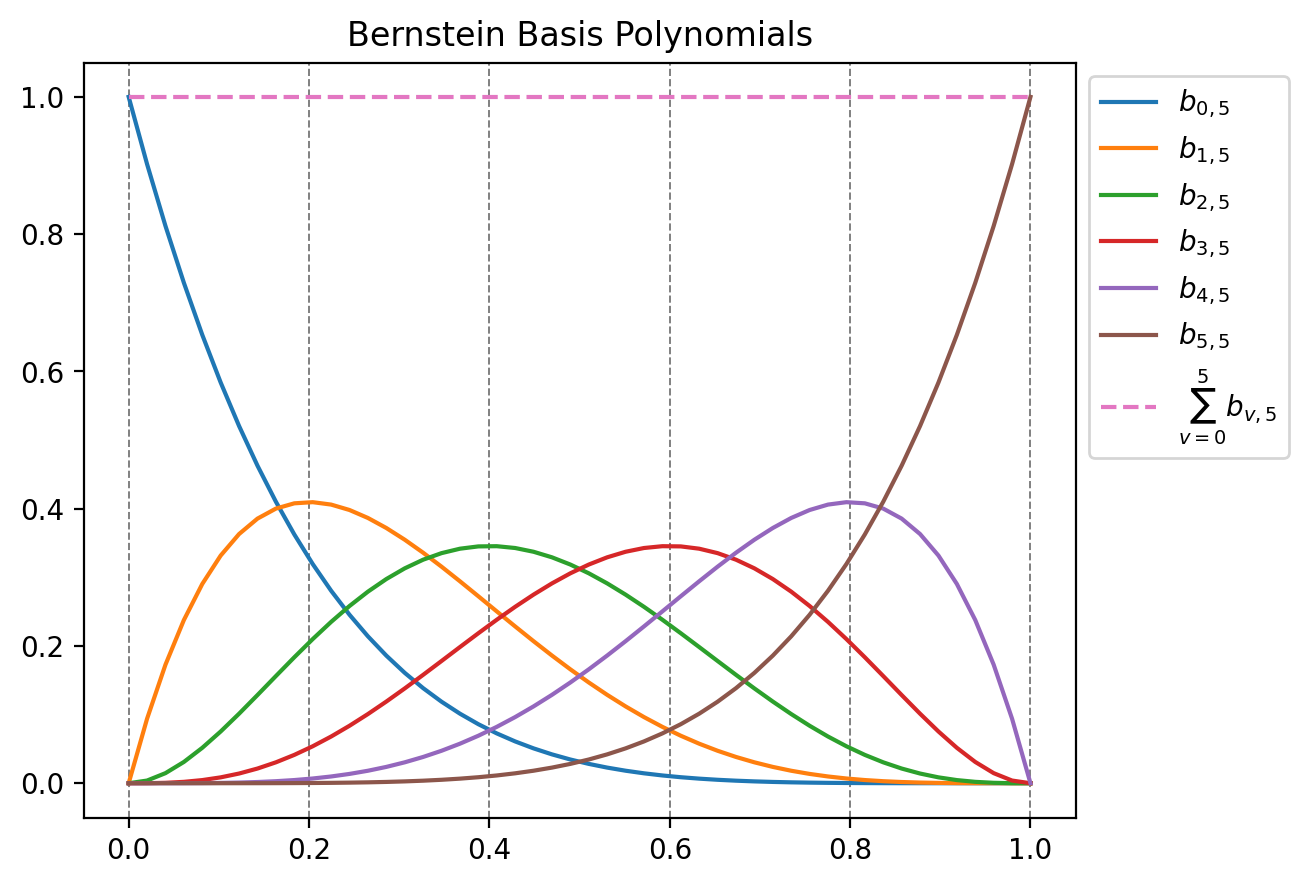
\includegraphics[width=0.5\textwidth]{a2-bernstein_basis_values.png}
    \caption{Bernstein Basis Values for $n=5$}
    \label{fig:bernstein-basis-plots}
    \small
        Fifth order bernstein basis values. Note how for different $x = \sfrac{v}{n}$ (where $v = 0,\dots,n$), the corresponding $b_{v,n}(x)$ peaks, which shows the weight of the control point being considered. Here, the $b_{v,n}(x)$ values are weights and the $f\left(\sfrac{v}{n}\right)$ could be theorized as control points (the above graph only has $b$).

        This figure can be generated by running the \texttt{src/bernstein\_basis.py} script as main.

        \textbf{Note}: The sum of all bernstein basis polynomials at any instance $x$ is 1.
\end{figure}

\subsubsection{Non-Holonomic Path using Bernstein Polynomials}

In a non-holonomic system, the system loses its ability to freely move in space due to some physical limitations. A differential drive robot (or a car) cannot move sideways, its non-holonomic constrain stems from the way velocity is resolved along its center, that is

\begin{equation}
    \dot{x} = v \cos(\theta) \quad 
    \dot{y} = v \sin(\theta) \quad\quad
    \Rightarrow \dot{y} = \dot{x} \tan(\theta) \quad
    \Rightarrow y = \int{\dot{x} \tan \left ( \theta \right ) dt}
    \label{eq:diffdrive-non-holo-constraint}
\end{equation}

The above integral cannot be computed directly, only numerical solutions to it exits. The kinematic model of a differential drive robot is given by

\begin{align*}
    \dot{q} = \begin{bmatrix}
        \dot{x} \\ \dot{y} \\ \dot{\theta}
    \end{bmatrix} = \begin{bmatrix}
    \cos(\theta) & 0 \\
    \sin(\theta) & 0 \\
    0 & 1
    \end{bmatrix} \begin{bmatrix}
    v \\ \omega
    \end{bmatrix}
\end{align*}

In the above equations, the point  $x, y, \theta$ is the robot position (in the 2D planar environment) and $v, \omega$ are the velocity commands given to the robot body.

Since the system above loses a degree of freedom - it cannot move in all possible directions in the neighborhood, in other words it is \emph{not} holonomic - only two of $x, y, \theta$ can be independently modeled.

\paragraph*{Problem Statement}
We are usually given the $x, y, \theta$ values at three points in time - the beginning $t_o$, waypoint $t_w$ or $t_c$, and end $t_f$. We are also given the first derivatives of $x$ at the time steps $t_o$, $t_c$, and $t_f$. We are also given $\dot{\theta}$ at time steps $t_o$ and $t_f$.
If this were holonomic (which it isn't), we could independently model the $x$, $y$, and $\theta$ as Bernstein polynomials and follow the given trajectory. But here, we have to use the constraint given by equation \ref{eq:diffdrive-non-holo-constraint}.

\subsubsection{Finding \texorpdfstring{$W_{x_i}$}{weights for x} and \texorpdfstring{$W_{k_i}$}{weights for k}}

We model the variable $x$ as

\begin{equation}
    x(t) \approx B_n(x)(t) = \sum_{i = 0}^{5} W_{x_i} B_i (\mu(t))
    \label{eq:x-bernstein-model}
\end{equation}

We model $\dot{x}$ as

\begin{equation}
    \dot{x}(t) = \sum_{i = 0}^{5} W_{x_i} \dot{B_i} (\mu(t))
    \label{eq:xdot-bernstein-model}
\end{equation}

We get the constraints as

\begin{align}
    \begin{bmatrix}
        x_o \\ x_w \\ x_f \\ 
        \dot{x}_o \\ \dot{x}_w \\ \dot{x}_f
    \end{bmatrix} = \begin{bmatrix}
        \sum_{i = 0}^{5} W_{x_i} B_i (\mu(t_o)) \\
        \sum_{i = 0}^{5} W_{x_i} B_i (\mu(t_w)) \\
        \sum_{i = 0}^{5} W_{x_i} B_i (\mu(t_f)) \\
        \sum_{i = 0}^{5} W_{x_i} \dot{B_i} (\mu(t_o)) \\
        \sum_{i = 0}^{5} W_{x_i} \dot{B_i} (\mu(t_w)) \\
        \sum_{i = 0}^{5} W_{x_i} \dot{B_i} (\mu(t_f))
    \end{bmatrix}
    \label{eq:wx-mat-equs-full}
\end{align}

These are 6 equations and 6 variables, giving the values of $W_{x_i}$ for $i \in [0\dots 5]$.

We model the variable $k = \tan(\theta)$

\begin{equation}
    \tan \left( \theta(t) \right) = k(t) \approx B_k(\mu(t)) = \sum_{i = 0}^{5} W_{k_i} B_i (\mu(t))
    \label{eq:tan-bernstein-model}
\end{equation}

Combining equations for $k$ and $\dot{x}$ models, we get

\begin{align}
    y(t) &= y_o + \int_{t_o}^{t} \left ( \sum_{i = 0}^{5} W_{x_i} \dot{B_i} (\mu(t)) \right ) \left ( \sum_{i = 0}^{5} W_{k_i} B_i (\mu(t)) \right ) dt 
    \nonumber\\
    &= y_o + \int_{t_o}^{t} \sum_{i=0}^{5} W_{k_i} \: f_i (t, t_0, t_f, W_{x_0}, \dots, W_{x_5}) \; dt
    \nonumber \\
    &= y_o + \sum_{i=0}^{5} W_{k_i} F_i (t, t_0, t_f, W_{x_0}, \dots, W_{x_5})
    \label{eq:t-mix-bernstein-model} \\
    f_i (t, t_0, t_f, W_{x_0}, \dots, W_{x_5}) &= B_i(\mu(t)) \sum_{i=0}^{5} W_{x_i} \dot{B}_i (\mu(t)) \nonumber
\end{align}

Note that the functions $f_i$ and $F_i$ are polynomials in $t$ (as we have calculated $W_{x_i}$ beforehand), and can be fully estimated beforehand.
Solve constraints like in equation \ref{eq:wx-mat-equs-full} for conditions on $y$ and $k = \tan(\theta)$. The solution will depend on the number and type of constraints.

\subsubsection{Bernstein Polynomials for Multi-robot UAVs}

For a multi-rotor robot, additional variables are needed. The variables will now be $x, y, z$ for the UAV's position in 3D Euclidean space, $\phi, \theta, \psi$ for the roll, pitch, and yaw orientation in 3D space.
The rotation matrix relating the global and vehicle inertial frame is given by

\begin{equation*} 
    \mathbf{R} = \begin{bmatrix}
        c\theta\,c\psi && c\theta\,s\psi && -s\theta \\
        s\phi\,s\theta\,c\psi-c\phi\,s\psi && s\phi\,s\theta\,s\psi + c\phi\,c\psi && s\phi c\theta \\
        c\phi\,s\theta\,c\psi && c\phi\,s\theta\,s\psi-s\phi\,c\psi && c\phi\,c\theta
    \end{bmatrix}
\end{equation*}

The vehicle's position, linear and angular velocity are represented by the following vectors

\begin{align*}
    \xi = [x\;\;y\;\;z]^\top && V = [u\;\;v\;\;w]^\top && \omega = [p\;\;q\;\;r]^\top
\end{align*}

The equations of motion are given by the following

\begin{align*}
    \dot{\xi} &= \mathbf{R}^{-1} V \\
    F &= m \dot{V} + \omega \times mV \\
    \begin{bmatrix}
        \dot{\phi} \\ \dot{\theta} \\ \dot{\psi}
    \end{bmatrix} &= \mathbf{E}^{-1} \begin{bmatrix}
        p \\ q \\ r
    \end{bmatrix} \\
    \mathbf{R} \begin{bmatrix}
        0 \\ 0 \\ mg
    \end{bmatrix} - \begin{bmatrix}
        0 \\ 0 \\ T
    \end{bmatrix} = \begin{bmatrix}
        F_{XB} \\ F_{YB} \\ F_{ZB}
    \end{bmatrix} &= m \begin{bmatrix}
        \dot{u} + qw - rv \\
        \dot{v} + ru - pw \\
        \dot{w} + pv - qu
    \end{bmatrix}
\end{align*}

These equations were taken from \cite{vilez2015trajectory}.

\subsubsection{Accommodating More Waypoints}

We could accommodate more waypoints through the following methods

\begin{enumerate}
    \item Increase the value of $n$ ($n$-th degree Bernstein basis). This will allow us to introduce more waypoints while keeping the system \emph{critically constrained}.
    \item We could directly add the waypoints, with the same $n$. This will make the system \emph{over-constrained}.
\end{enumerate}

\paragraph{Piece-wise Bernstein Polynomials}

However, we usually have a global path planner (like RRT) running at lower frequencies (say $10$ Hz). That path planner gives many points (consider them to be waypoints, with the exception of start and goal).

At a different frequency, and within a small neighborhood, we need to travel from one point to another (on this proposed solution by the global path planner) through waypoints. This is done through a piece-wise fitting of Bernstein Polynomials while keeping the end constraints in check (for position and velocity).

Through this method, we can theoretically accommodate all the points proposed by the global path planner into a big piece-wise Bernstein polynomial.

\subsubsection{Collision Avoidance}

If there is a static obstacle, we can do one of the following things

\begin{itemize}
    \item \textbf{Break the Bernstein path}: We can Break the Bernstein/Bezier path into smaller Bernstein basis polynomials and in the segment containing the obstacle, place a waypoint sufficiently far away from the obstacle. We must keep the end trajectory conditions in check, so that we do not give different velocities for the ends.
    \item We can optimize for a waypoint using an optimization formulation (similar to the multiple robot formulation in the next subsection).
\end{itemize}

\paragraph{Multiple Non-holonomic Robots}

We can selectively optimize coefficients for bernstein polynomials of different robots so that they avoid collisions. The main concepts are derived from \cite{klanvcar2010case} (a summary can be found in \cite{skrjanc2007cooperative}). Consider a Bernstein polynomial with $b = 4$ degree. The polynomial will be given by

\begin{equation}
    \mathbf{r}(\lambda) = \sum_{i=0}^{b} B_{i, b} (\lambda) \: \mathbf{p}_i \qquad \textup{where} \; B_{i, b} (\lambda) = \: ^{b}\textup{C}_i \: \lambda^i \: (1-\lambda)^{b-i} \;,\; i = 0, 1, \dots, b
\end{equation}

Where $\mathbf{r} = [x\;\;y]^\top$ is the path. The points $\mathbf{p}_i = [x_i\;\;y_i]^\top$ are the control points.
The normalized time is given by $\lambda(t) = t/T_{\textup{max}}$.
Considering the first derivative of path (the velocity), we get

\begin{equation}
    \mathbf{v}(\lambda) = \frac{d \mathbf{r}(\lambda)}{d \lambda} = b \sum_{i = 0}^{b-1} \left ( \mathbf{p}_{i+1} - \mathbf{p}_i \right ) B_{i, b-1} (\lambda)
\end{equation}

Here $\mathbf{v}(\lambda) = [v_x,\:v_y]^\top$. We also know that $B_{b-1, i}(0) = 0 \:, i = 1, \dots, b-1$ while $B_{b-1, 0}(0) = 1$. We also know that $B_{b-1, i}(1) = 0 \:, i = 0, \dots, b-2$ which $B_{b-1, b-1}(1) = 1$.
This means that $\mathbf{v}(0) = 4(\mathbf{p}_1 - \mathbf{p}_0)$ and $\mathbf{v}(1) = 4(\mathbf{p}_4 - \mathbf{p}_3)$. 
These give us the values for $\mathbf{p}_1$ and $\mathbf{p}_3$ readily as follows

\begin{align}
    \mathbf{p}_1 = \mathbf{p}_0 + \frac{1}{4} \mathbf{v}(0) &&
    \mathbf{p}_3 = \mathbf{p}_4 - \frac{1}{4} \mathbf{v}(1)
\end{align}

We already know that $\mathbf{p}_0$ is the starting point and $\mathbf{p}_4$ is the ending point. This means that we have $\mathbf{p}_2$ to optimize for each robot, to avoid a collision.

\paragraph{Multiple robots}

Let us consider a case with multiple robots, each with a trajectory given by $\mathbf{r}_i(\lambda_i) = \left[ x_i(\lambda_i), y_i(\lambda_i) \right]^\top$. Note that each robot can have its own normalized time reference given by $\lambda_i = t/T_{\textup{max}_i}$.
The distance between two robots $i$ and $j$ is given by $r_{ij}(t) = |\mathbf{r}_i(t) - \mathbf{r}_j(t)|$. We must keep this above a certain threshold $d_s$ (minimum distance between two robots).
We would also like to minimize the length of the paths of each robot. The length of path of robot $i$ is given by

\begin{equation}
    s_i = \int_0^1 \left ( v_{xi}^2 (\lambda_i) + v_{yi}^2 (\lambda_i) \right )^{\sfrac{1}{2}} d\lambda_i
\end{equation}

Note that the above equation is a variable \emph{only} in $\mathbf{p}_{2i}$ (which is $\mathbf{p}_2$ for robot $i$). We can theoretically minimize this and get $\mathbf{p}_{2i}$ from this itself (keeping collision avoidance and other things aside). But this doesn't guarantee anything other than the shortest path length.

\paragraph{Optimization problem}

We will now consider minimizing the collective path lengths, while adhering to the constraints. This gives the following optimization objective

\begin{align*}
    &\textup{min} \sum_{i=1}^{n} s_i
    \\
    &\textup{subject to} \;\; d_s - r_{ij}(t) \leq 0 \:,\: \; 
    v_i(t) - v_{\textup{max}_i} \:,\: a_i(t) - a_{\textup{max}_i} \leq 0
    \;
    \forall \: i,j,i \neq j \;,\; 0 \leq t \leq \textup{max}_i (T_{\textup{max}_i})
\end{align*}

This can be converted to the following optimization problem

\begin{align}
    \begin{split}
        F =& \sum_{i} s_i + c_1 \sum_{ij} \textup{max}_{ij} (0,\: \sfrac{1}{r_{ij}(t)} - \sfrac{1}{d_s}) + c_2 \sum_i \textup{max}_i (0,\: v_i(t) - v_{\textup{max}_i}) \\
        & + c_3 \sum_{i} \textup{max}_i (0,\: a_i(t) - a_{\textup{min}_i})
    \end{split} 
    \nonumber \\
    &\textup{min} \qquad F
    \nonumber \\
    &\textup{subjected to} \quad \mathbf{P}_2,\: \mathbf{T}_{\textup{max}}
    \nonumber \\
    & i, j, i \neq j,\;\; 0 \leq t \leq \textup{max}_i (T_{\textup{max}_i})
\end{align}

The values $c_1$, $c_2$, and $c_3$ are scalar constants in the above equation. The $c_1$ term ensures no collision, the $c_2$ term ensures maximum possible velocity, and the $c_3$ term ensures maximum acceleration. Due to the latter two, the penalty function $F$ is also subjected to the time for each robot.
The above equations can probably be solved through an optimizer like \href{https://docs.scipy.org/doc/scipy/reference/generated/scipy.optimize.minimize.html}{scipy.optimize.minimize}.

\subsubsection{Results}

The videos can be found \href{https://iiitaphyd-my.sharepoint.com/:f:/g/personal/avneesh_mishra_research_iiit_ac_in/EogE243Ab4lDvm5VSueCLY8B7tLHOWnVw8i8PQnv5Bndfg?e=k8xJ1n}{here}.

\begin{figure}[ht]
    \centering
    \begin{subfigure}[b]{0.3\textwidth}
        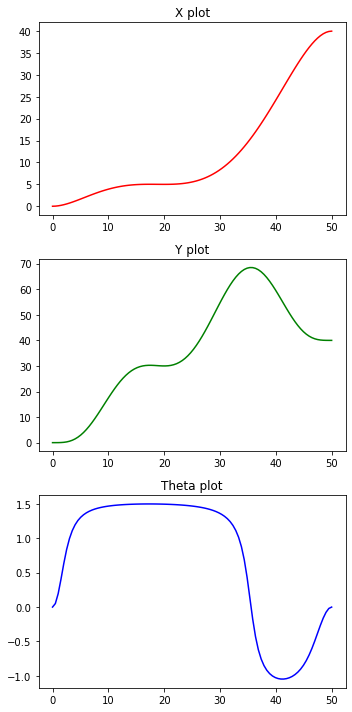
\includegraphics[width=\textwidth]{a2-out-1.png}
        \caption{Plots for $x$, $y$, and $\theta$}
    \end{subfigure}
    \begin{subfigure}[b]{0.6\textwidth}
        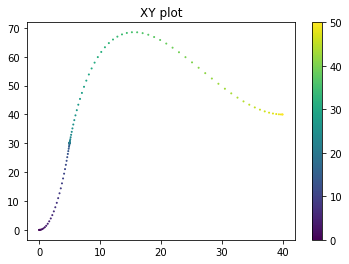
\includegraphics[width=\textwidth]{a2-out-1-xy.png}
        \caption{Plot for $x, y$ path}
    \end{subfigure}
    \caption{Case 1 trajectories}
    \label{fig:case-1-traj}
    \small
        File name is \texttt{out\_1.avi}. As it can be seen, the constraints for the `dx` at waypoint is being adhered (the vehicle comes to a stop there). It'll be more beneficial to not stop at waypoints.
\end{figure}

\begin{figure}
    \centering
    \begin{subfigure}[b]{0.25\textwidth}
        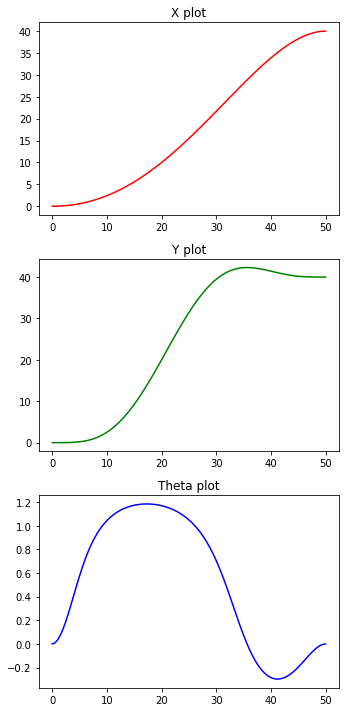
\includegraphics[width=\textwidth]{a2-out-2.png}
        \caption{Plots for $x$, $y$, and $\theta$}
    \end{subfigure}
    \begin{subfigure}[b]{0.5\textwidth}
        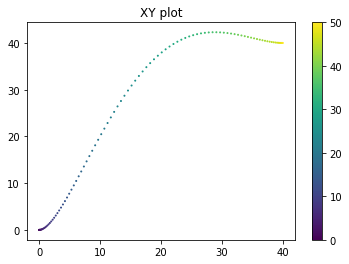
\includegraphics[width=\textwidth]{a2-out-2-xy.png}
        \caption{Plot for $x, y$ path}
    \end{subfigure}
    \caption{Case 2 trajectories}
    \label{fig:case-2-traj}
\end{figure}

\begin{figure}
    \centering
    \begin{subfigure}[b]{0.25\textwidth}
        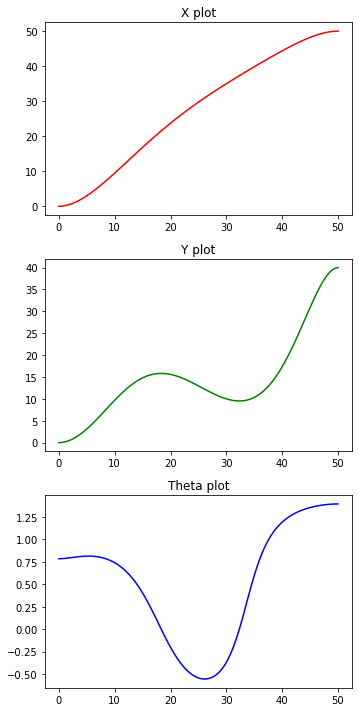
\includegraphics[width=\textwidth]{a2-out-3.png}
        \caption{Plots for $x$, $y$, and $\theta$}
    \end{subfigure}
    \begin{subfigure}[b]{0.5\textwidth}
        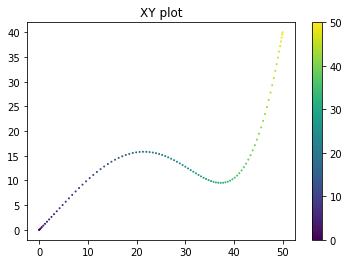
\includegraphics[width=\textwidth]{a2-out-3-xy.png}
        \caption{Plot for $x, y$ path}
    \end{subfigure}
    \caption{Case 3 trajectories}
    \label{fig:case-3-traj}
    \small
        Avoiding obstacles by moving the waypoints of bernstein polynomials.
\end{figure}

\begin{figure}
    \centering
    \begin{subfigure}[b]{0.3\textwidth}
        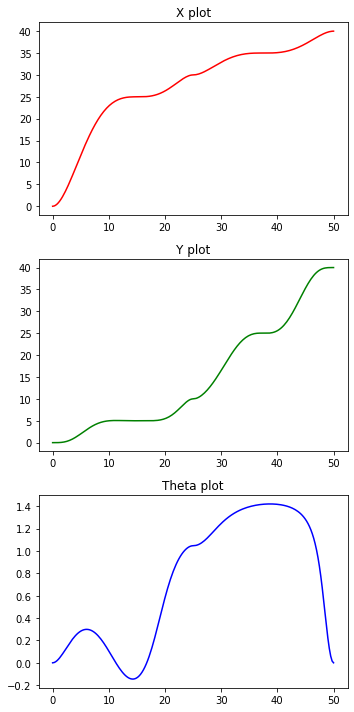
\includegraphics[width=\textwidth]{a2-out-4.png}
        \caption{Plots for $x$, $y$, and $\theta$}
    \end{subfigure}
    \begin{subfigure}[b]{0.5\textwidth}
        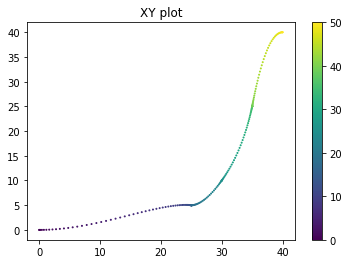
\includegraphics[width=\textwidth]{a2-out-4-xy.png}
        \caption{Plot for $x, y$ path}
    \end{subfigure}
    \caption{Case 4 trajectories}
    \label{fig:case-4-traj}
    \small
        Avoiding obstacles by joining two bernstein polynomials.
\end{figure}

\paragraph{Advantages of Bernstein Polynomials}

Bernstein polynomials have the following advantages over other methods

\begin{enumerate}
    \item It has smooth blending through the waypoints. This means that not only the function is continuous, and differentiable; but also its derivatives are continuous and differentiable.
    \item It can be quickly calculated, given a set of waypoints. If we do not want to solve any equations, we directly set the waypoints as control points.
    \item Applying a Euclidean transformation to the entire path is equivalent to applying the transformation to the control points alone. The weighed sum only depends on time (not space).
\end{enumerate}
